% How Fast Do Agents Rot? — empirical study of long-horizon degradation in LLM agents.
% Written in standard article-class LaTeX so it compiles without a venue style file;
% to target COLM, drop in colm2024_conference.sty and switch \documentclass.
\documentclass[11pt]{article}
\usepackage[utf8]{inputenc}
\usepackage{microtype}
\usepackage{amsmath,amssymb}
\usepackage{graphicx}
\usepackage{booktabs}
\usepackage{array}
\usepackage{xcolor}
\usepackage[hidelinks]{hyperref}
\usepackage[round]{natbib}
\usepackage[margin=1in]{geometry}
\usepackage{titlesec}
\titlespacing*{\section}{0pt}{1.2em}{0.5em}
\titlespacing*{\subsection}{0pt}{0.9em}{0.35em}

\newcommand{\rstep}{r}            % per-step reliability symbol
\newcommand{\horizon}{H}

\title{\textbf{How Fast Do Agents Rot? An Empirical Study of\\ Long-Horizon Degradation in LLM Agents}}
\author{}
\date{}

\begin{document}
\maketitle

\begin{abstract}
Agent benchmarks report steadily rising success rates, yet deployed LLM agents
remain unreliable on long, multi-step tasks. We argue this tension is largely an
artifact of \emph{horizon}: benchmarks score agents at task lengths where success
is still high, while production demands far longer horizons. We measure the effect
directly. Across 5{,}625 controlled agent trajectories spanning five open models
(1.2B--671B parameters, three vendor families), three task families, five task
horizons ($H\!\in\!\{2,4,8,16,32\}$ dependent steps), and three context regimes, we
characterize the \emph{shape} of degradation and disentangle its cause. We find that
task success follows a geometric law, $P(\text{success})\approx a\,\rstep^{\horizon}$,
where $\rstep$ is a model- and task-specific per-step reliability: the best-fitting
shape is geometric in $10/15$ model$\times$task cells. Per-step reliability rises with
model scale (Pearson $r{=}0.38$ vs.\ $\log$ parameters) but never reaches $1$ on
non-trivial tasks, so geometric compounding guarantees collapse at long horizons even
for the strongest model. Degradation moreover \emph{accelerates}: per-step accuracy
falls from $0.49$ early in a trajectory to $0.35$ late, a super-geometric tail.
Disentangling step-count from context-length, we find the rot is \emph{intrinsic to
executing many dependent steps}, not raw context length: bounding the context window
(compressed regime) and collapsing the task to a single long prompt (padded regime)
\emph{both} steepen decay relative to the natural agent loop ($p{<}0.05$), ruling out
``lost-in-the-middle'' as the driver and showing that naive context truncation
backfires. Projecting measured per-step reliability onto the horizons of popular
benchmarks shows the gap concretely: mean projected success falls from $0.31$ at
GAIA-length tasks to $0.18$ at SWE-bench-length to $0.10$ at $100$-step production
horizons. We release all code, prompts, seeds, and raw trajectories.
\end{abstract}

\section{Introduction}
Large language model (LLM) agents---models that perceive context, plan, call tools,
and update state in a loop---now score highly on a fast-growing suite of benchmarks
\citep{jimenez2024swebench,yao2024taubench,zhou2023webarena,mialon2023gaia}. The
trajectory of reported numbers is encouraging, and the time horizon of tasks models
can complete has been doubling rapidly \citep{kwa2025metr}. Yet practitioners who
deploy agents report a stubborn gap: agents that pass benchmark tasks remain
unreliable on the long, open-ended workflows that production demands.

We take a specific position on why. A benchmark task has a \emph{horizon}: the number
of dependent steps an agent must execute correctly. If each step succeeds
independently with probability $\rstep<1$, then a task of horizon $\horizon$ succeeds
with probability $\approx \rstep^{\horizon}$---a quantity that is close to $\rstep$ for
short tasks but collapses geometrically as $\horizon$ grows. Benchmarks predominantly
sample short-to-medium horizons; production agents operate at horizons an order of
magnitude longer. If degradation is geometric, then \emph{benchmarks systematically
sample the flat top of the decay curve}, and the production gap is not noise but an
expected consequence of horizon.

This paper tests that hypothesis empirically. Rather than a single number, we
characterize the \emph{law}---the functional form of success versus horizon---and
\emph{disentangle its cause}, separating the number of sequential steps from the
length of accumulated context. We make four contributions:
\begin{enumerate}
\item \textbf{A measured law of horizon decay.} On controlled, oracle-verifiable agent
  tasks, success follows a geometric law $P\approx a\,\rstep^{\horizon}$ (best fit in
  $10/15$ model$\times$task cells; \S\ref{sec:law}). The single quantity $\rstep$
  (per-step reliability) governs everything.
\item \textbf{Degradation accelerates.} Per-step accuracy itself declines as a
  trajectory lengthens ($0.49\!\to\!0.35$ from the first to the last third),
  producing a super-geometric tail (\S\ref{sec:accel}).
\item \textbf{Cause: step count, not context length.} Using three context regimes that
  break the natural collinearity of steps and tokens, we show that bounding context
  and collapsing to a single prompt both \emph{worsen} decay relative to the natural
  agent loop. The rot is intrinsic to executing many dependent steps; lost-in-the-
  middle is not the driver, and naive context truncation backfires (\S\ref{sec:cause}).
\item \textbf{The benchmark gap, quantified.} Projecting measured $\rstep$ onto the
  horizons of popular agent benchmarks makes the gap concrete: success that looks
  moderate at benchmark horizons collapses at production horizons (\S\ref{sec:gap}).
\end{enumerate}
Our study is deliberately reproducible: synthetic tasks with exact oracles (no
LLM-judge noise), five public models, recorded seeds, and a released dataset. This
paper is the empirical companion to a survey of agent failure modes; where that work
argues benchmarks miss long-horizon failure, this work measures it.

\section{Related Work}
\textbf{Agent benchmarks.} A large family of benchmarks evaluates agents on software
issues \citep{jimenez2024swebench}, tool-and-user interaction
\citep{yao2024taubench,barres2025tau2bench}, web navigation
\citep{zhou2023webarena,deng2023mind2web}, general assistance \citep{mialon2023gaia},
operating-system and app control \citep{xie2024osworld,trivedi2024appworld},
function calling \citep{patil2025bfcl}, multi-environment agent suites
\citep{liu2024agentbench}, and end-to-end company workflows \citep{xu2024agentcompany}. These report aggregate single-attempt success and span
short to very long horizons, but rarely report a horizon-resolved decay curve or a
reliability metric. \citet{kwa2025metr} track the \emph{time horizon} of completable
tasks over model generations; we instead fix the models and resolve success
\emph{against} horizon within a controlled environment.

\textbf{Evaluation validity and reliability.} \citet{kapoor2024agents} document
cost-blindness and evaluation shortcomings in agent benchmarking, and
\citet{zhu2025abc} establish best practices for rigorous agentic benchmarks. Both
motivate reliability-oriented, horizon-aware measurement. \citet{cemri2025mast} build
a taxonomy of multi-agent failures. Our compounding result gives a quantitative basis
for one of their core observations: local errors cascade.

\textbf{Long context and compounding.} A complementary line studies how models use
long contexts: degradation with input position \citep{liu2024lostmiddle}, with input
length at fixed task \citep{levy2024moretokens}, and on synthetic long-context probes
\citep{hsieh2024ruler,modarressi2025nolima}. \citet{dziri2023faithfate} show that
transformer accuracy decays rapidly with compositional task complexity, and
\citet{laban2025lostconv} show large drops from single- to multi-turn settings. These
predict that \emph{context length} should drive agent degradation. Our disentangling
experiment tests this directly and finds the opposite for our tasks: bounding context
worsens performance, implicating step count rather than context length.

\textbf{Agent methods.} ReAct-style reasoning-and-acting \citep{yao2023react} and
verbal self-reflection \citep{shinn2023reflexion} are the dominant agent loops; our
harness uses a ReAct-style structured loop. We study the unmodified loop to measure
intrinsic degradation rather than the effect of a particular mitigation.

\section{Method}\label{sec:method}
\subsection{Task families}
We use three synthetic task families, each a tool-using agent loop with a
ground-truth simulator that verifies success \emph{exactly} (no LLM judge). All three
have a single horizon knob $\horizon$ = the number of dependent operations, and
$O(1)$--$O(k)$ per-step state so that step count and context length can be varied
independently (\S\ref{sec:regimes}). Each family stresses a distinct capability:
\begin{itemize}
\item \textbf{ledger} (arithmetic working memory): maintain three account balances
  through $\horizon$ deposit/withdraw/transfer operations; report a queried balance.
\item \textbf{refchain} (long-range retrieval): track the current value of one
  announced variable through $\horizon$ assignments interleaved with distractor
  variables and re-assignments; report its final value.
\item \textbf{cipher} (procedural execution): apply $\horizon$ ordered string edits
  (swap/rotate/replace) to a 5-character string; report the final string.
\end{itemize}
At each step the agent receives one instruction and must emit a single JSON object
carrying its updated running state; no correctness feedback is given, so per-step
errors compound and are measured. After $\horizon$ steps the environment poses the
final query. The simulator scores each submitted state and the final answer against
the oracle, yielding per-trajectory success, per-step accuracy, and the first-error
step.

\subsection{Context regimes: disentangling step count from context length}\label{sec:regimes}
At a fixed horizon the \emph{number of operations is held equal} across three regimes,
which vary only the two axes of interest:
\begin{center}
\begin{tabular}{lcc}
\toprule
regime & agent turns & context length \\
\midrule
natural    & $\horizon$ & long (full history) \\
compressed & $\horizon$ & \textbf{short} (carried state, windowed history) \\
padded     & \textbf{1} & long (all $\horizon$ operations in one prompt) \\
\bottomrule
\end{tabular}
\end{center}
Comparing \emph{natural vs.\ compressed} (same turns, different context length)
isolates the context-length effect; \emph{natural vs.\ padded} (same information,
different number of turns) isolates the multi-step-process effect. The same underlying
task instance is reused across regimes, making the comparison paired.

\subsection{Models, design, and metrics}
We evaluate five open instruction-tuned models served via OpenRouter, spanning
$1.2$B--$671$B parameters and three vendor families:
Llama-3.2-1B, Qwen2.5-7B, Llama-3.1-8B, Llama-3.3-70B, and DeepSeek-V3.
The full design is $5\text{ models}\times3\text{ families}\times5\text{ horizons}
\times3\text{ regimes}\times25\text{ trials}=5{,}625$ trajectories. Generation
temperature is fixed at $0.2$; seeds are recorded per trajectory. We report
per-cell success with Wilson 95\% intervals, fit decay curves and select among
geometric/threshold/linear shapes by AIC, estimate per-step reliability $\rstep$
directly as the fraction of individual steps correct, and fit a logistic model
$\mathrm{logit}\,P=\beta_0+\beta_H\log_2\!\horizon\cdot C(\text{regime})$ for the
disentangling analysis. We pre-registered the hypotheses, design, and analysis plan
before the full run; deviations are logged in the released repository.

\section{Results}
\subsection{Degradation follows a geometric law}\label{sec:law}
Figure~\ref{fig:decay} shows success versus horizon for every model and family.
Success declines monotonically with horizon wherever the task is non-trivial for the
model. Fitting geometric ($P=a\,\rstep^{\horizon}$), threshold (logistic-in-$\horizon$),
and linear forms and selecting by AIC, the \textbf{geometric form wins in $10$ of $15$}
model$\times$family cells; the remaining $5$ are threshold-shaped---visible in
Figure~\ref{fig:decay} as the ``cliff'' where strong models hold near-perfect accuracy
on \texttt{ledger} until $\horizon{=}32$. The geometric law is therefore the dominant
description, and per-step reliability $\rstep$ is the quantity that governs it.

Crucially, the magnitude of decay is governed by $\rstep$, which varies with both model
and task difficulty (Table~\ref{tab:rstep}). On \texttt{refchain} (variable tracking)
the strong models have $\rstep\!\approx\!1$ and show essentially no decay---a
\emph{ceiling}; on \texttt{cipher} (procedural string edits) even DeepSeek-V3 has
$\rstep{=}0.25$ and collapses within a few steps. The same models thus appear robust
or fragile depending entirely on per-step reliability, exactly as $P\approx
\rstep^{\horizon}$ predicts. This is the central point: whether degradation is
\emph{visible} depends on $\rstep$ and the horizon sampled, but $\rstep<1$ on any
non-trivial task makes collapse at long horizon inevitable.

\begin{figure}[t]
\centering
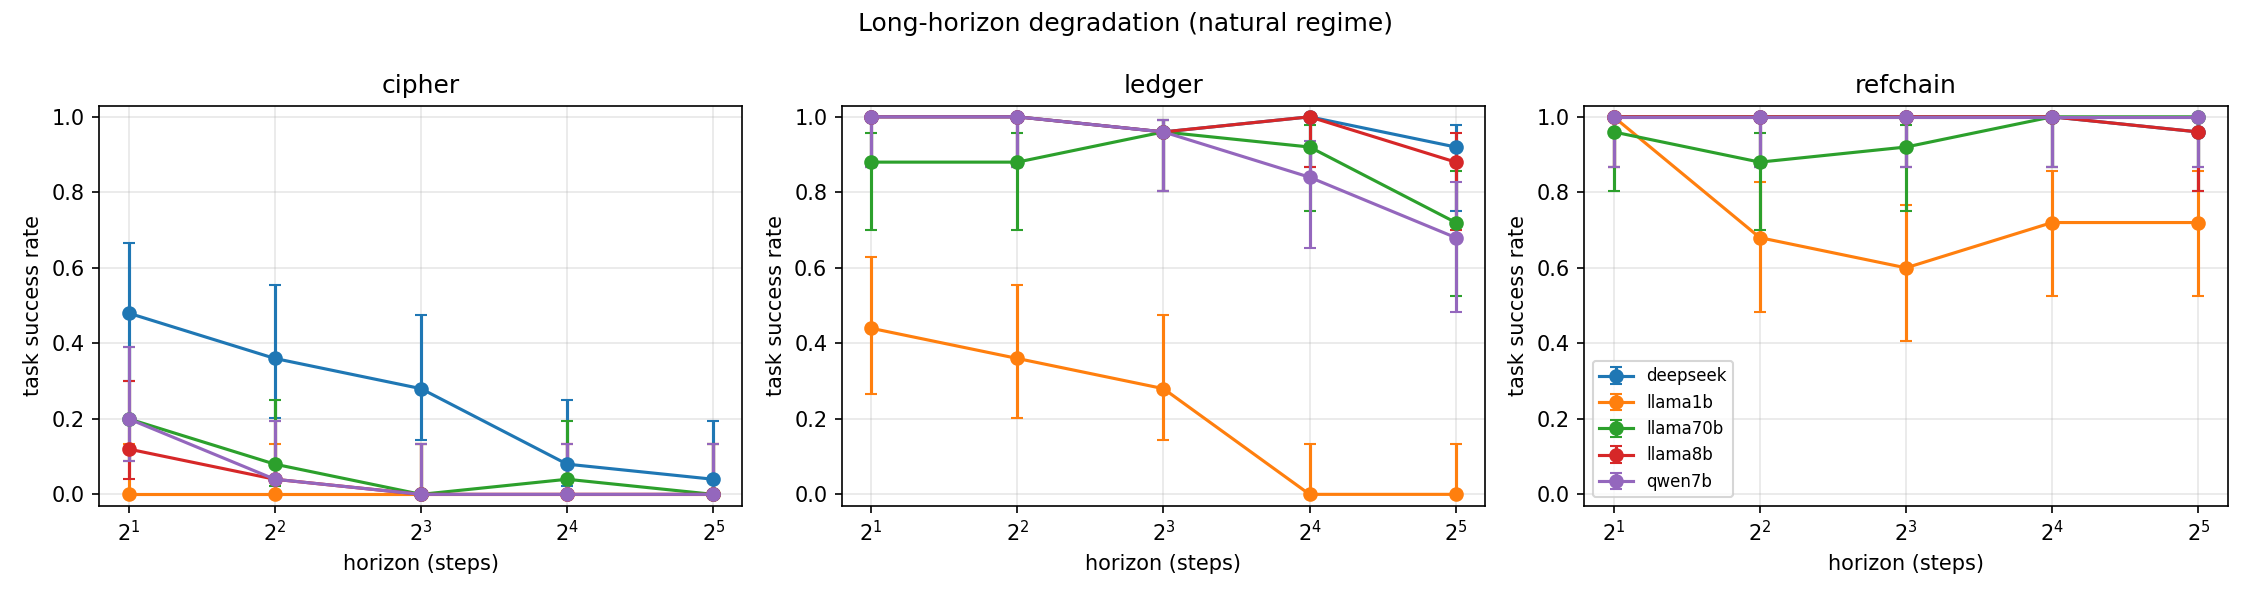
\includegraphics[width=\textwidth]{../figures/fig1_decay_curves.png}
\caption{Task success vs.\ horizon (natural regime), per task family, per model
(Wilson 95\% intervals; horizon on a $\log_2$ axis). Decay is steep where per-step
reliability is low (\texttt{cipher}), a long-horizon cliff at medium difficulty
(\texttt{ledger}), and a ceiling where reliability is near-perfect (\texttt{refchain},
strong models). All are consistent with $P\approx \rstep^{\horizon}$.}
\label{fig:decay}
\end{figure}

\begin{table}[t]
\centering
\small
\begin{tabular}{lccccc}
\toprule
& \multicolumn{5}{c}{success rate at horizon $\horizon$ (natural, families pooled)} \\
model ($\sim$params) & $\horizon{=}2$ & $4$ & $8$ & $16$ & $32$ \\
\midrule
Llama-3.2-1B (1.2B)  & 0.48 & 0.35 & 0.29 & 0.24 & 0.24 \\
Qwen2.5-7B (7.6B)    & 0.73 & 0.68 & 0.65 & 0.61 & 0.56 \\
Llama-3.1-8B (8B)    & 0.71 & 0.68 & 0.65 & 0.67 & 0.61 \\
Llama-3.3-70B (70B)  & 0.68 & 0.61 & 0.63 & 0.65 & 0.57 \\
DeepSeek-V3 (671B)   & 0.83 & 0.79 & 0.75 & 0.69 & 0.64 \\
\bottomrule
\end{tabular}
\caption{Success decays monotonically with horizon for every model. Larger models
start higher and decay more gently, but all decay.}
\label{tab:decay}
\end{table}

\begin{table}[t]
\centering
\small
\begin{tabular}{lccc}
\toprule
& \multicolumn{3}{c}{per-step reliability $\rstep$ (natural)} \\
model & cipher & ledger & refchain \\
\midrule
Llama-3.2-1B  & 0.00 & 0.10 & 0.38 \\
Qwen2.5-7B    & 0.06 & 0.74 & 0.99 \\
Llama-3.1-8B  & 0.02 & 0.91 & 1.00 \\
Llama-3.3-70B & 0.09 & 0.79 & 0.94 \\
DeepSeek-V3   & 0.25 & 0.94 & 0.98 \\
\bottomrule
\end{tabular}
\caption{Per-step reliability spans the full range by task and model. cipher is hard
per-step, refchain easy, ledger intermediate---yet the geometric law holds across all.
Per-step reliability rises with model scale (Pearson $0.38$ vs.\ $\log$ params).}
\label{tab:rstep}
\end{table}

\subsection{Per-step reliability rises with scale---but never to 1}
Across the $1.2$B--$671$B ladder, per-step reliability rises with model size: the
Pearson correlation between $\rstep$ and $\log_{10}$ parameters is $+0.38$, and the
within-family Llama trend climbs from $0.16$ (1B) to $0.64$ (8B) before saturating at
$0.61$ (70B). DeepSeek-V3 is most reliable at $0.72$. Scale thus buys per-step
reliability with diminishing returns, but no model reaches $\rstep{=}1$ on the
non-trivial families. Because success compounds as $\rstep^{\horizon}$, even the best
model is guaranteed to fall below any fixed reliability target at a sufficiently long
horizon; scale moves the cliff, it does not remove it.

\subsection{Degradation accelerates within a trajectory}\label{sec:accel}
A pure geometric law assumes a \emph{constant} per-step hazard. We find the hazard
instead \emph{rises} as a trajectory lengthens: pooling long-horizon trajectories,
mean per-step accuracy falls from $0.49$ in the first third of a trajectory to $0.35$
in the last third (Figure~\ref{fig:perstep}). The first error lands, on average, about
a third of the way through; once an agent errs it rarely recovers, consistent with
prior reports that models ``get lost'' after a wrong turn \citep{laban2025lostconv}.
Acceleration makes the true decay \emph{super-geometric}---worse than the constant-
hazard model---so geometric fits, if anything, understate long-horizon collapse.

\begin{figure}[t]
\centering
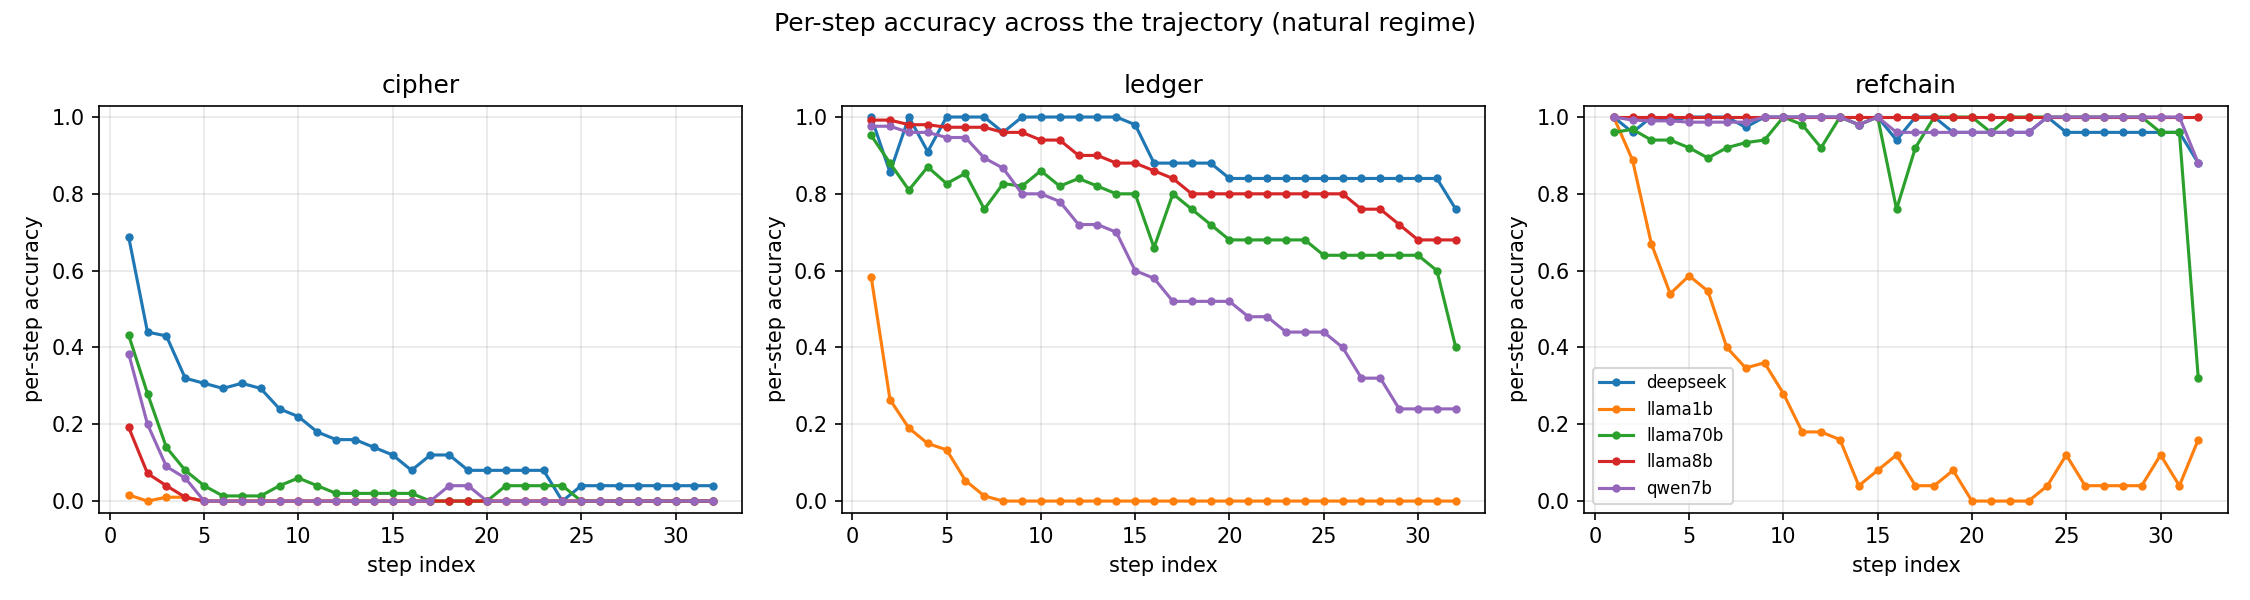
\includegraphics[width=\textwidth]{../figures/fig3_perstep_accuracy.png}
\caption{Per-step accuracy vs.\ step index within a trajectory (natural regime). Accuracy
declines as the trajectory progresses: the per-step hazard rises, giving a
super-geometric tail rather than constant-hazard geometric decay.}
\label{fig:perstep}
\end{figure}

\subsection{The driver is step count, not context length}\label{sec:cause}
Figure~\ref{fig:regime} contrasts the three context regimes. The \emph{natural} agent
loop---full history, one step per turn---is the \emph{best} regime at every horizon
(pooled success $0.69\!\to\!0.53$ from $\horizon{=}2$ to $32$). Both interventions are
worse: \emph{compressed} (bounded context, $0.54\!\to\!0.21$) and \emph{padded}
(single long prompt, $0.46\!\to\!0.22$). Fitting
$\mathrm{logit}\,P=\beta_0+\beta_H\log_2\!\horizon\cdot C(\text{regime})$, the decay
slope per horizon doubling is $-0.37$ (natural), $-0.62$ (compressed, $p{=}0.0007$ vs.\
natural), and $-0.53$ (padded, $p{=}0.023$). \textbf{Both manipulations steepen decay;
neither flattens it.}

This is decisive for the cause. If raw context length drove degradation
(lost-in-the-middle), bounding the context window would \emph{help}; instead it
hurts---models rely on their accumulated reasoning history, and truncating it removes
a scaffold they depend on. If the multi-step process were the problem, collapsing the
task into a single prompt would help; instead it also hurts---one-shot execution of
$\horizon$ operations forgoes the per-step externalization that the agent loop
provides. What remains is that degradation is \emph{intrinsic to executing many
dependent steps}: the number of operations, not how they are packaged, is what
compounds. A direct practical corollary: naive context truncation, a common
production tactic, \emph{backfires} on these models.

\begin{figure}[t]
\centering
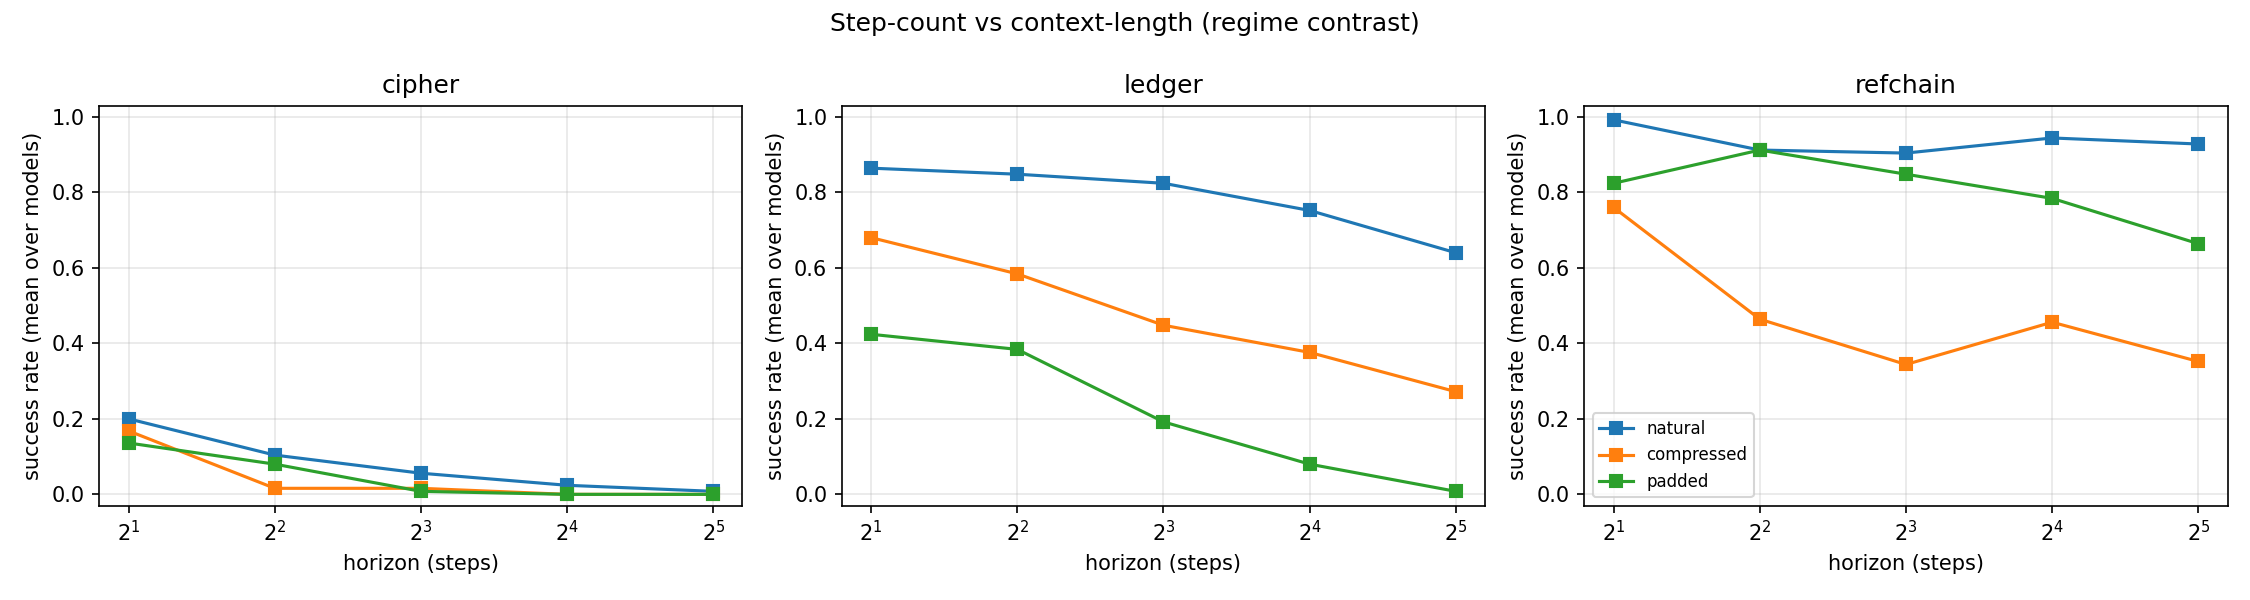
\includegraphics[width=\textwidth]{../figures/fig2_regime_contrast.png}
\caption{Step-count vs.\ context-length. At fixed horizon the number of operations is
held equal across regimes. The natural loop (full context, step-by-step) is best;
bounding context (compressed) and collapsing to one prompt (padded) both steepen
decay. Degradation is intrinsic to step count, not context length.}
\label{fig:regime}
\end{figure}

\subsection{Mechanism}
Beyond success, the harness records how trajectories fail. Format and tool-call drift
---a turn whose output cannot be parsed as a valid action---rises with horizon and
reaches $21\%$ of trajectories overall, an instance of the interface-level failures
agents are known to exhibit. The first-error position concentrates around the first
third of the trajectory, and per-step accuracy never recovers afterward
(\S\ref{sec:accel}): errors are absorbing. Together these give a mechanistic picture
of ``rot'': a per-step error rate that is non-zero, rises over time, propagates
silently---no oracle interrupts a plausible-but-wrong intermediate state, much as
hallucinated content survives without a verifier \citep{huang2025hallucination}---and
compounds into trajectory-level failure.

\subsection{The benchmark gap, quantified}\label{sec:gap}
The practical payoff is to place real benchmarks on the decay curve. Using the mean
fitted per-step reliability ($\rstep{=}0.55$) and the geometric law, we project task
success at the representative horizons of popular benchmarks (Table~\ref{tab:gap}).
Projected success falls from $0.31$ at GAIA-length tasks ($\sim 8$ steps) to $0.18$ at
SWE-bench-length ($\sim 30$ steps) to $0.10$ at a $100$-step production horizon. The
absolute numbers depend on our task mix, but the \emph{shape} is the point: an agent
that looks moderately reliable at benchmark horizons is far less reliable at the
horizons production actually requires. Benchmarks sample the flat top of a curve that
collapses out of frame.

\begin{table}[t]
\centering
\small
\begin{tabular}{lcc}
\toprule
benchmark (representative horizon, steps) & projected success \\
\midrule
GAIA ($\sim$8)              & 0.31 \\
WebArena ($\sim$15)        & 0.24 \\
$\tau$-bench ($\sim$20)    & 0.21 \\
SWE-bench / OSWorld ($\sim$30) & 0.18 \\
TheAgentCompany ($\sim$100) & 0.10 \\
\bottomrule
\end{tabular}
\caption{Projecting measured per-step reliability ($\rstep{=}0.55$) onto
representative benchmark horizons. Horizons are order-of-magnitude task lengths from
the cited benchmark papers; they place each benchmark on the curve rather than asserting
its exact score.}
\label{tab:gap}
\end{table}

\section{Discussion and recommendations}
Our results recast the agent-reliability gap as a predictable consequence of horizon.
Three takeaways follow. \textbf{For practitioners:} estimate per-step reliability
$\rstep$ on your own tasks and treat the achievable horizon as $\log(\text{target})/
\log \rstep$; because the hazard accelerates, budget below the geometric estimate.
Do not reach for naive context truncation as a reliability fix---in our data it
worsens decay; the model relies on its history. \textbf{For benchmark designers:}
report success \emph{resolved against horizon}, not a single aggregate, and include
horizons beyond the comfortable regime; a horizon-decay curve is far more predictive
of production behavior than a point estimate. \textbf{For the field:} per-step
reliability is the right primitive for agent evaluation. It is cheap to measure,
composes multiplicatively into task success, and---unlike aggregate pass rates---
extrapolates across horizons.

\section{Limitations and threats to validity}
Our tasks are synthetic and chosen for exact verifiability and a clean horizon knob;
they trade ecological validity for control. We mitigate this by spanning three
difficulty regimes and by framing the benchmark projection (\S\ref{sec:gap}) as a
placement on the curve rather than a literal score for any benchmark. We study five
open models up to $671$B parameters; the largest proprietary models may have higher
$\rstep$, but our scaling analysis indicates this moves the cliff rather than removing
it, and $\rstep<1$ on hard tasks suffices for the argument. Per-step reliability for
the \texttt{cipher} family is low enough that some cells are near the floor; we report
per-step accuracy and Wilson intervals throughout so floor/ceiling effects are visible.
Hosted inference carries residual non-determinism despite fixed temperature and seeds;
we record seeds and release raw outputs. Three small models (Llama-3.2-3B, Gemma-3-4B,
Phi-4-mini) were excluded because their hosted routes did not adhere to the structured
protocol (empty tool-call or conversational responses); this is itself a mild instance
of interface-level fragility but limits the density of the small-model ladder.

\section{Conclusion}
Agents rot geometrically. Task success follows $P\approx \rstep^{\horizon}$ in a per-step
reliability $\rstep$ that rises with scale but never reaches $1$ on non-trivial tasks,
so long horizons guarantee collapse; the decay moreover accelerates within a
trajectory. The driver is the number of dependent steps, not context length---bounding
context makes things worse, not better. Because benchmarks sample short horizons, they
report the flat top of this curve and hide the collapse that defines production
behavior. Measuring and reporting per-step reliability against horizon would close much
of the gap between what we benchmark and what we deploy.

\paragraph{Reproducibility.} All code, task generators, prompts, seeds, raw
trajectories, and analysis scripts are released. Every quantitative claim in this paper
traces to the released dataset.

\bibliographystyle{plainnat}
\bibliography{references}
\end{document}
